\chapter*{}\addcontentsline{toc}{part}{\IntroductionName}
\vspace{-1.5cm}
    \begin{minipage}[r]{.95\textwidth}\raggedleft
    \HUGE\bfseries\IntroductionName
    \end{minipage}
\vspace{2.5cm}

\noindent
                    %%%%%%%%%%%%%%%%%%%%%%%%%%%%                  (EDIT BELOW)

\begin{quote}
  {
    \raggedleft
    \textit{"I've been using Vim for about 2 years now,\\mostly because I can't figure out how to exit it."}\\

    \raggedleft
    \textbf{\href{https://x.com/iamdevloper/status/435555976687923200}{I Am Developer}}\\
  }
\end{quote}

This book is a printed version of my Neovim Tips plugin that can be found on Github at
\href{https://github.com/saxon1964/neovim-tips}{saxon1964/neovim-tips}.

\begin{figure}[h]
  \centering
  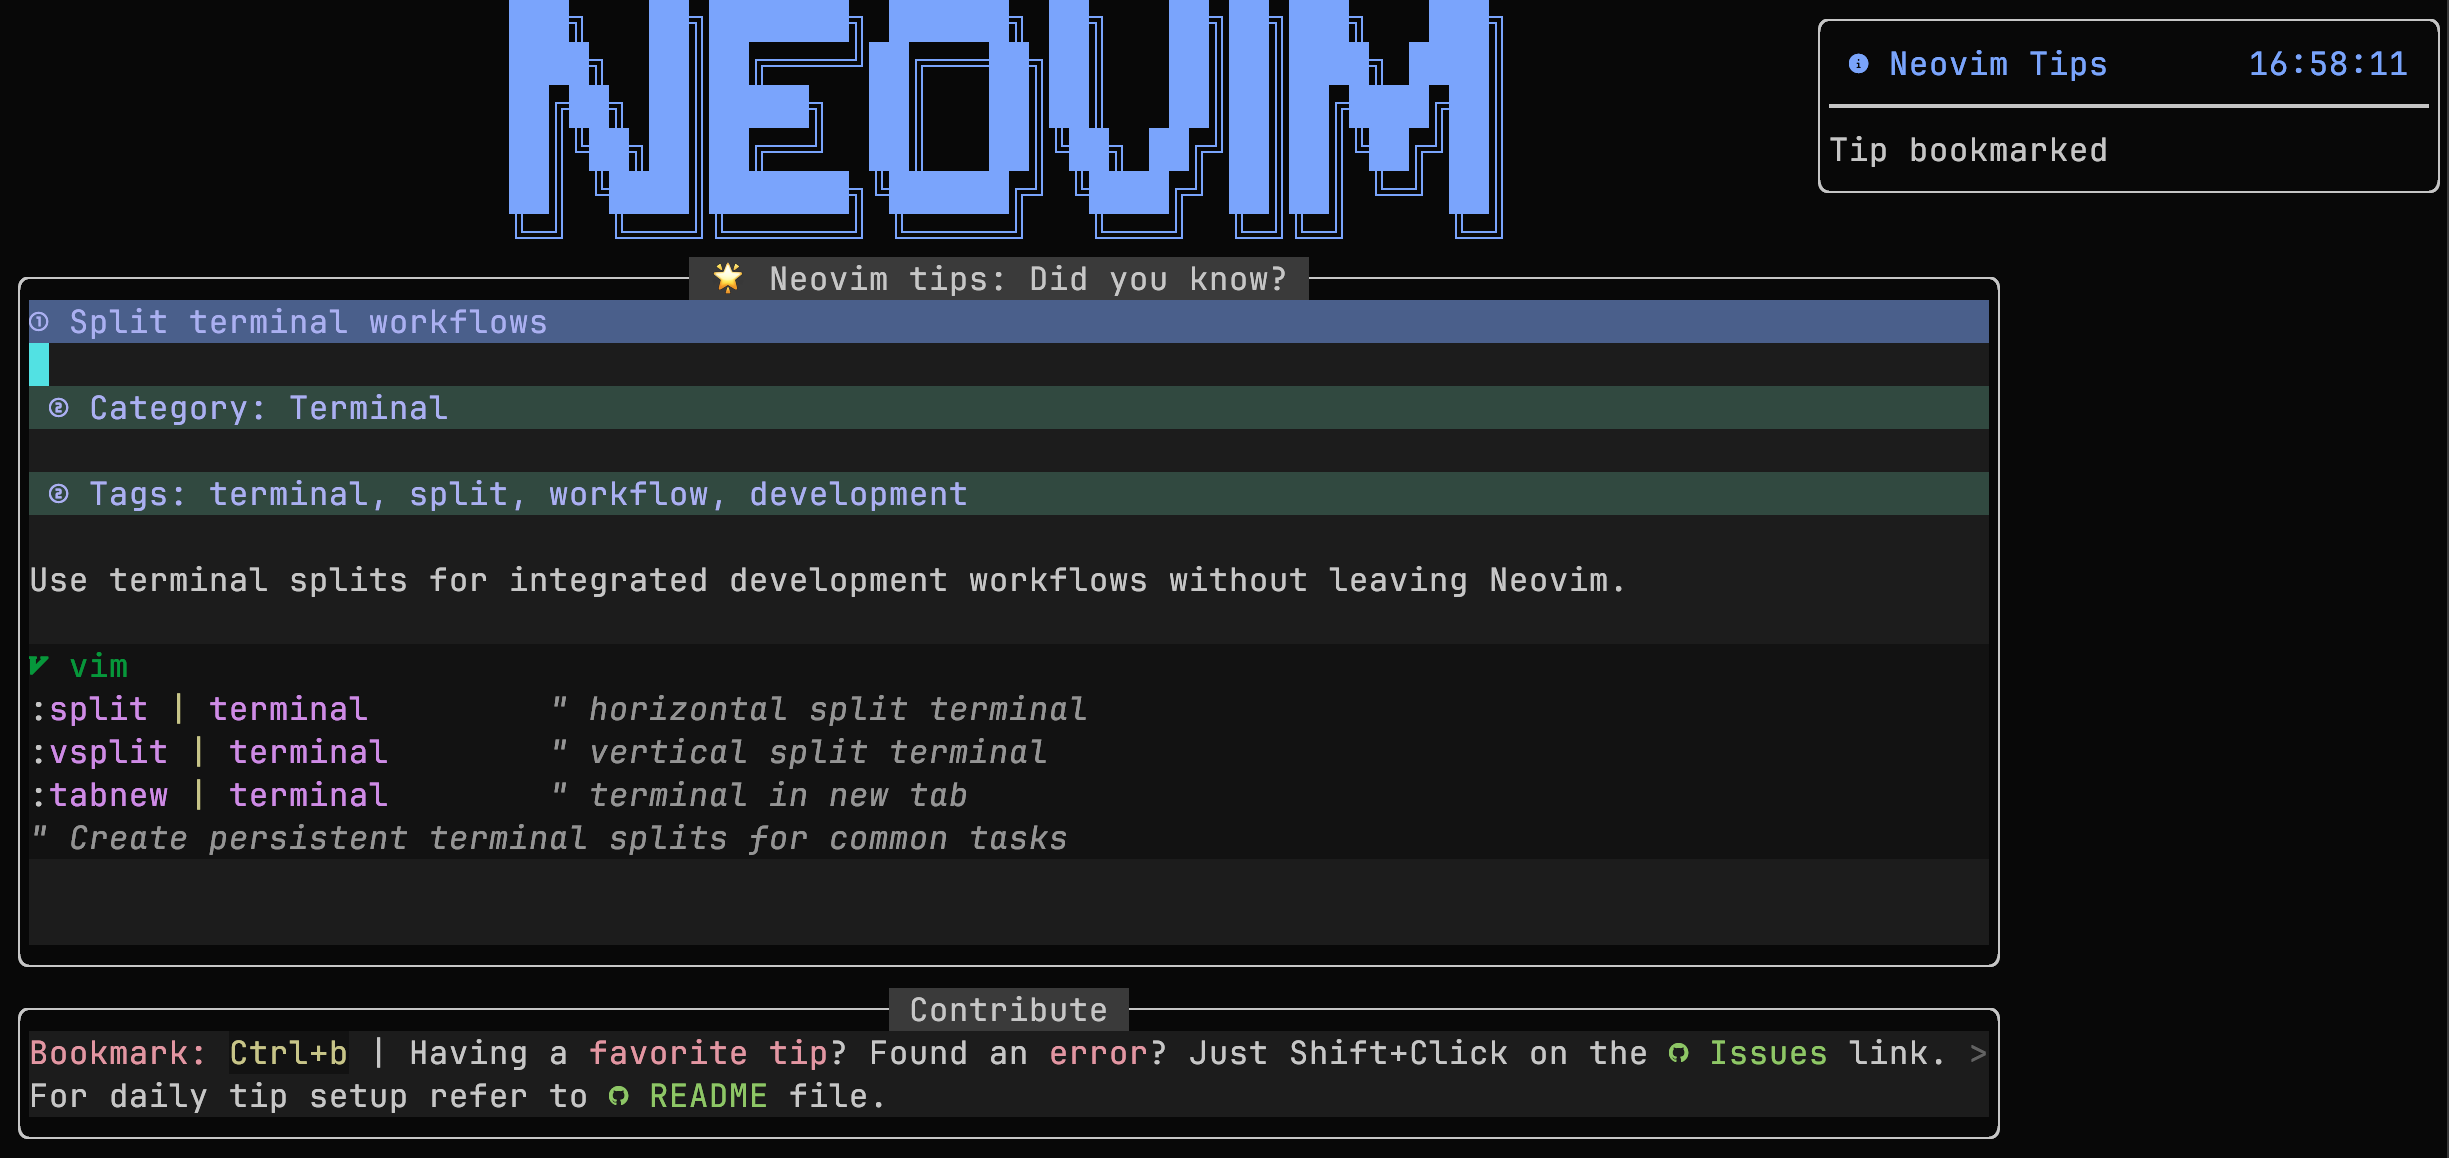
\includegraphics[width=\textwidth]{Structure/Images/s1.png}
  \vspace{-2em}
  \caption*{Daily tip from Neovim Tips plugin}
\end{figure}

This Lua plugin for Neovim brings together hundreds of helpful tips, tricks, and shortcuts, all available through a custom picker. It's easy to expand with your own entries, so the collection grows with you and your workflow.

I started to work on this little plugin because I love neovim and I still remember how difficult it was to learn the basic commands. This book, together with the plugin, should help you to learn some basic (:wq, write and quit) and some not so basic commands (ddp, move line down) related to Neovim.

I have provided a solid initial batch of tips and if you have your favorite one that is not listed, I will be happy to include it in the next release with proper credits. \href{mailto:smalltux@yahoo.com}{Send your commands, tips and tricks to me}, create an issue or submit a pull request. Usign the plugin, you can also add your own tips and tricks that will be stored on your local computer, you don't have to share anything with me. A few plugin screenshots can be found on the following page.

\begin{figure}[h]
  \centering
  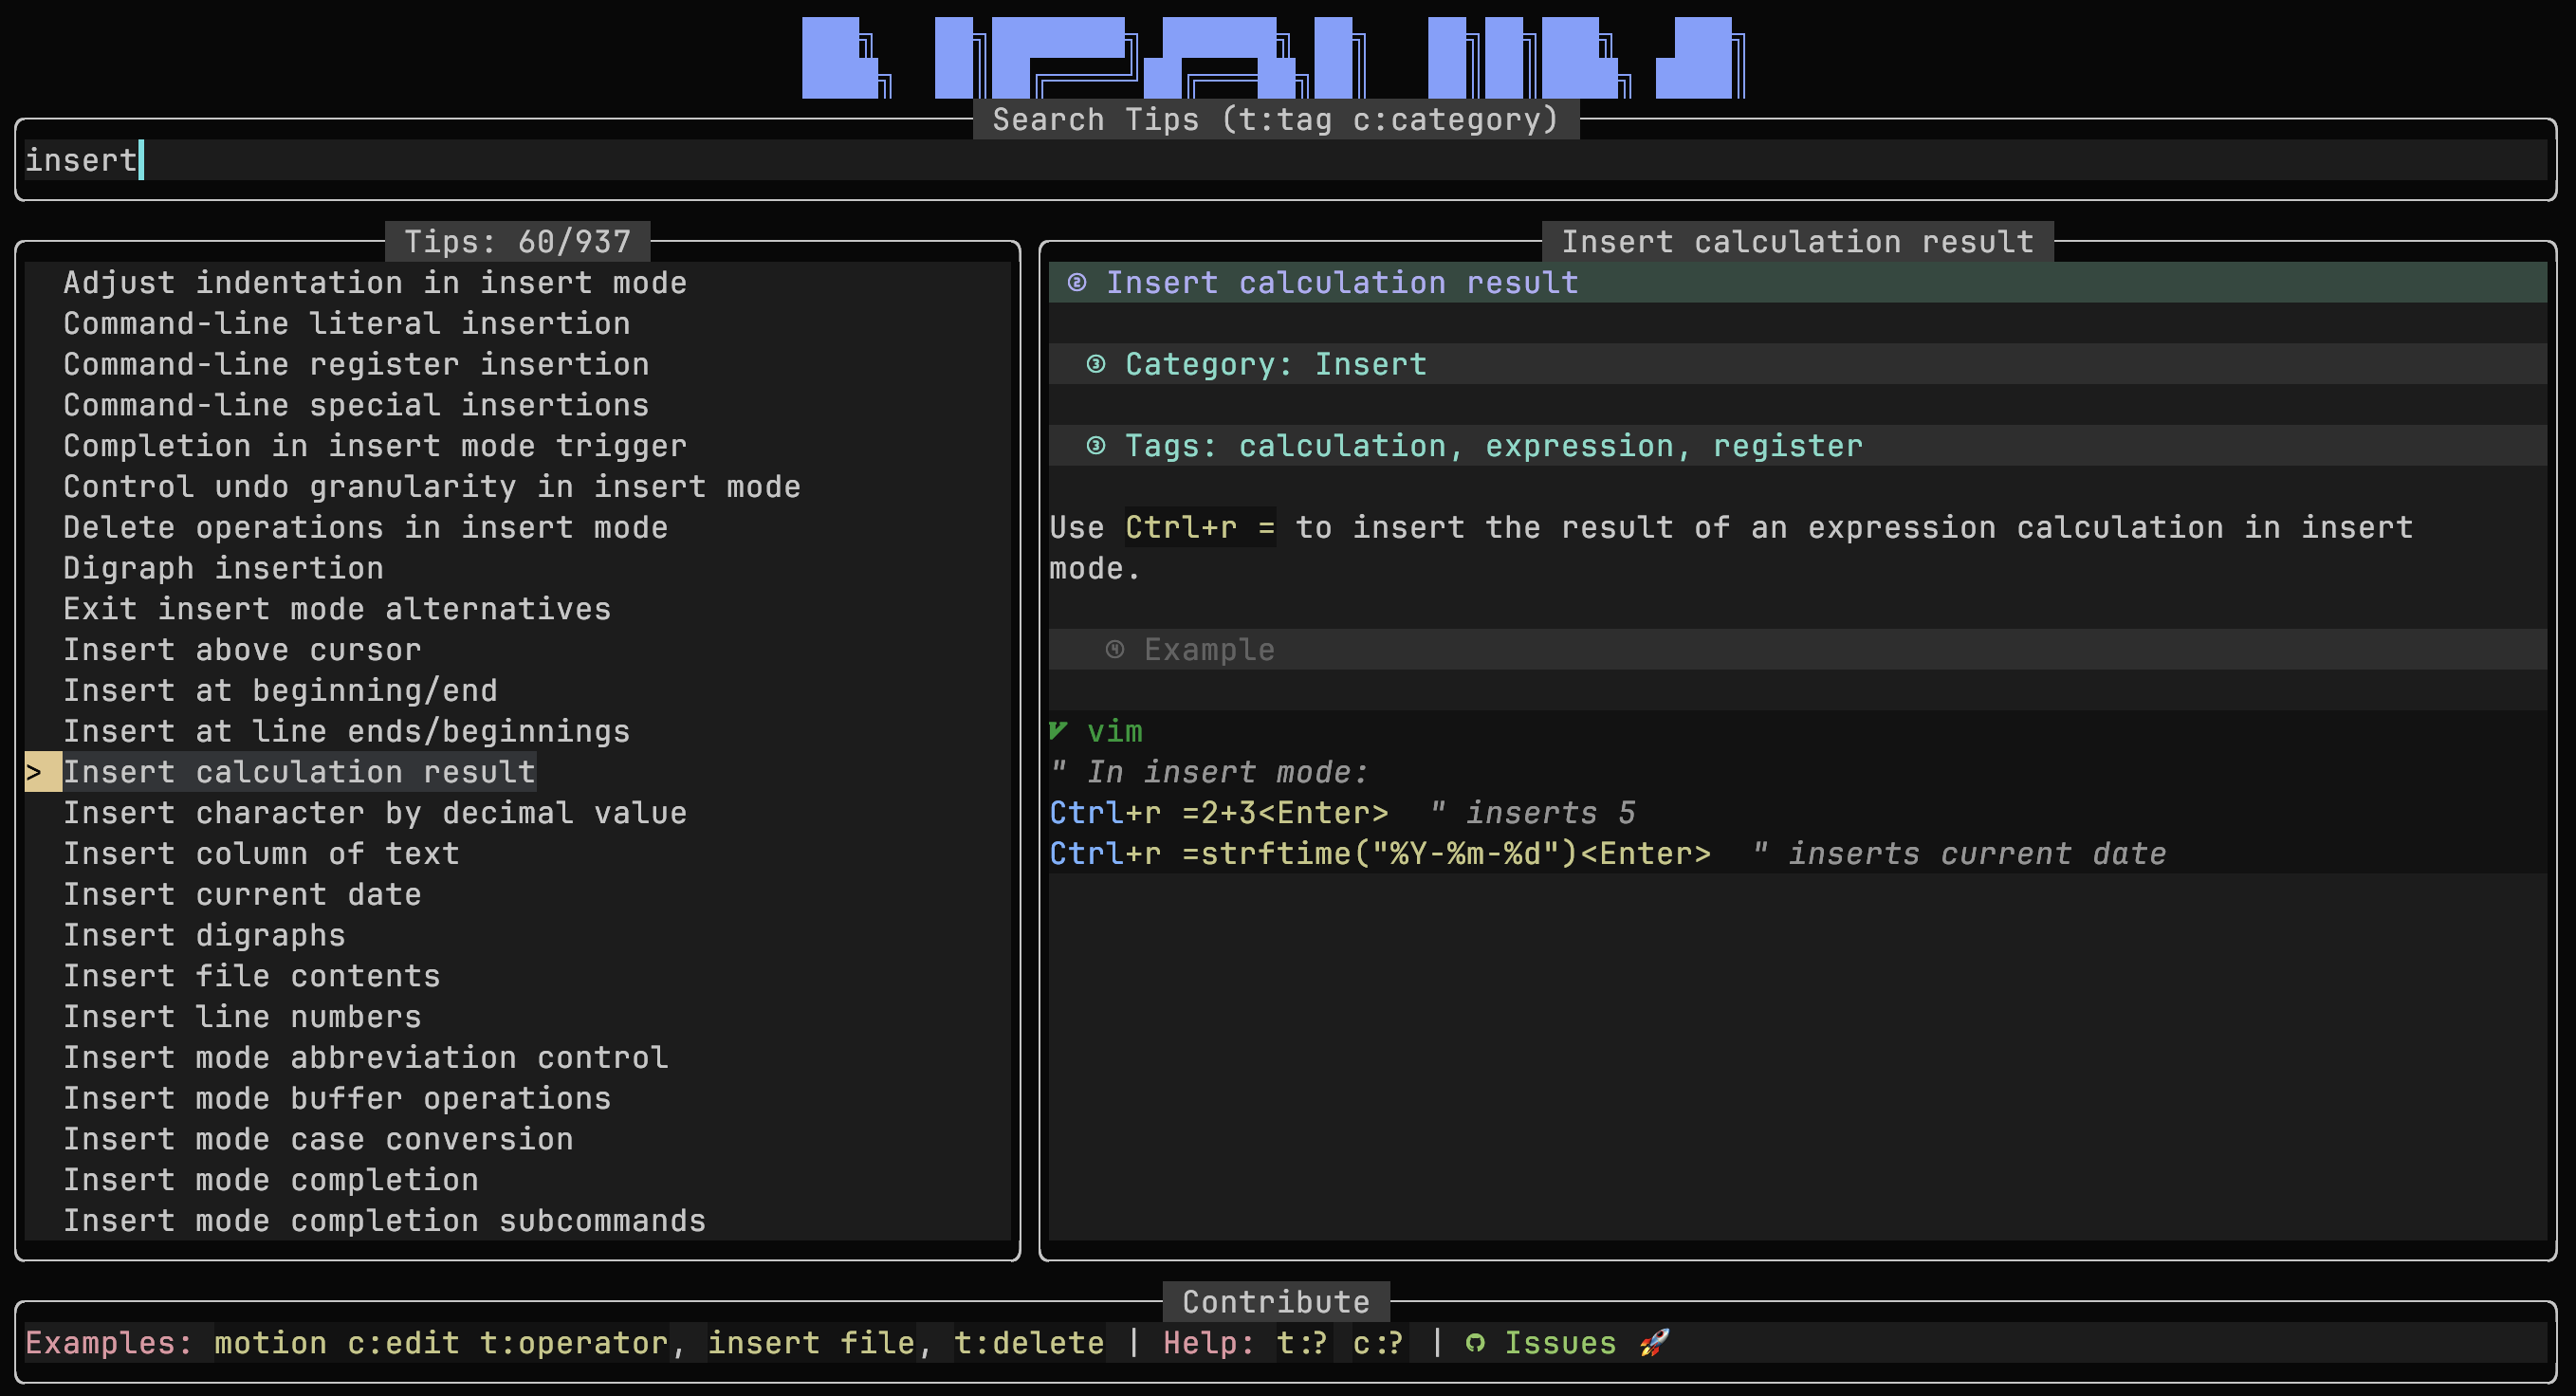
\includegraphics[width=\textwidth]{Structure/Images/s2.png}
  \vspace{-2em}
  \caption*{Neovim Tips plugin screenshot}
\end{figure}

\vspace{1cm}

This book is dedicated to my son \textbf{Luka} who learned me to use and love Neovim.
\clearpage
